\documentclass[12pt]{article}
%\usepackage[utf8]{inputenc}
%\documentclass[UTF8]{ctexart}
%\usepackage[UTF8, heading = false, scheme = plain]{ctex}
\usepackage{geometry}
%geometry{a4paper,scale=0.9}
\geometry{a4paper,left=1cm,right=1cm,top=1cm,bottom=2cm}
\usepackage{amsfonts}
\usepackage{color}
\usepackage{url}
%\usepackage{biblatex}
\usepackage{amsmath}
\usepackage{amssymb}
\usepackage{latexsym}
\usepackage{cite}
%\addbibresource{ref.bib}
%\bibliography{ref.bib}
\usepackage{caption}
\usepackage{graphicx, subfig}
\usepackage{float}
%\usepackage[fontset=ubuntu]{ctex}
%\usepackage{fontspec}
\usepackage{xeCJK}
%\usepackage[colorlinks,
%anchorcolor=black,
%citecolor=black]{hyperref}
%\setmainfont{SimSun}
\usepackage[section]{placeins}
\usepackage{enumitem}
\usepackage{framed}
\usepackage[framemethod=TikZ]{mdframed}
\usepackage{indentfirst}
\usepackage{setspace}%使用间距宏包
\linespread{1.5}
%\title{预备知识}
%\author{leolinuxer }
%\date{June 2020}

\begin{document}
%\maketitle
\section{常见函数的导数}
$$ f(x) = \ln{x} \qquad f'(x) = \frac{1}{x} $$

$$ f(x) = \log_ax \qquad f'(x) = \frac{1}{x\ln{a}} $$

\section{泰勒公式}
一阶泰勒公式展开为:
$$ f(x) = f(a) + f'(a)(x-a) $$

\subsection{泰勒公式和梯度下降法的关系}
根据一阶泰勒公式,有:
$$ f(\theta) \approx f(\theta_0) + (\theta - \theta_0) \cdot \nabla f(\theta_0) $$

其中,$\theta - \theta_0$ 是微小矢量,它的大小是的步进长度$\eta$,所以 $\theta - \theta_0 = \eta v$,其中 $v$ 是矢量。

我们希望每次 $\theta$ 更新,都能让函数 $f(\theta)$ 减小,也就是说,我们希望 $f(\theta) < f(\theta_0)$,那么有:

$$ f(\theta) - f(\theta_0) \approx \eta v \cdot \nabla f(\theta_0) < 0 $$

因为 $\eta$ 为标量,且一般设定为正值,所以可以忽略,所以有:
$$ v \cdot \nabla f(\theta_0) < 0$$

在这个不等式中,$v$ 和 $\nabla f(\theta_0) $ 都是矢量,$\nabla f(\theta_0)$ 是当前位置的梯度方向,$v$ 是下一步前进的单位方向,是需要求解的,有了它,就可以确定 $\theta$ 了。

两个向量 $A B$ 的乘积为:
$$ A \cdot B = |A||B|cos(\alpha)$$
要使两个向量的乘积小于零,只要 $cos(\alpha) = -1$,即两个向量反向,所以可以知道:
$$ v = - \frac{\nabla f(\theta_0)}{|\nabla f(\theta_0)|}$$

带入到 $\theta - \theta_0 = \eta v$ 中,有:
$$ \theta = \theta_0 - \eta \frac{\nabla f(\theta_0)}{|\nabla f(\theta_0)|}$$

因为 $|\nabla f(\theta_0)|$ 是标量,可以合并到 $\eta$ 中,所以可以得到:
$$ \theta = \theta_0 - \eta \nabla f(\theta_0)$$

\section{似然函数}
\subsection{似然函数概述}
在数理统计学中,似然函数是一种关于统计模型中的参数的函数,表示模型参数中的似然性。“似然性”与“或然性”或“概率”意思相近,都是指某种事件发生的可能性,但是在统计学中,“似然性”和“或然性”或“概率”又有明确的区分。

概率:用于在已知一些参数的情况下,预测接下来的观测所得到的结果。

似然性:用于在已知某些观测所得到的结果时,对有关事物的性质的参数进行估计。在这种意义上,{\color{red} 似然函数可以理解为条件概率的逆反。}

{\color{red} 总结:概率是已知参数,预测观测结果;似然性是已知观测结果,估计参数。}

\subsection{似然函数的定义\cite{Zhihu-likelihood}}
似然函数是给定联合样本值$x$下关于(未知)参数 $\theta$ 的函数,即:$L(\theta|x) = f(x|\theta)$。

这里的小 $x$ 是指联合样本随机变量 $X$ 取到的值,即 $X = x$;

这里的 $\theta$ 是指未知参数,它属于参数空间;

这里的 $f(x|\theta)$ 是一个密度函数,特别地,它表示(给定)$\theta$下关于联合样本值$x$的联合密度函数。

所以从定义上,似然函数和密度函数是完全不同的两个数学对象。:前者是关于 $\theta$ 的函数,后者是关于$x$ 的函数。所以这里的等号 $=$ 理解为函数值形式的相等,而不是两个函数本身是同一函数(根据函数相等的定义,函数相等当且仅当定义域相等并且对应关系相等)。

\subsection{\color{red}似然函数和概率的联系}
(1) 如果 $X$ 是离散的随机向量,那么其概率密度函数 $f(x|\theta)$可改写为 $f(x|\theta) = \mathbb{P}_{\theta}(X=x)$,即代表了在参数 $\theta$ 下,随机向量 $X$ 取到值 $x$ 的可能性;并且,如果我们发现:
$$ L(\theta_1|x) = \mathbb{P}_{\theta_1}(X=x) > \mathbb{P}_{\theta_2}(X=x) = L(\theta_2|x)  $$
那么似然函数就反应出这样一个朴素推测:\textbf{在参数$\theta_1$下随机向量$X$取到值$x$的可能性大于在参数$\theta_2$下随机向量$X$取到值$x$的可能性。换句话说,我们更有理由相信(相对于$\theta_2$来说)$\theta_1$更有可能是真实值。这里的可能性由概率来刻画。}

(2)如果$X$是连续的随机向量,那么其密度函数 $f(x|\theta)$ 本身(如果在$x$连续的话)在$x$处的概率为0,为了方便考虑一维情况:给定一个充分小 $\epsilon > 0$,那么随机变量$X$取值在 
$$ \mathbb{P}(x-\epsilon < X < x+\epsilon) = \int_{x-\epsilon}^{x+\epsilon}f(x|\theta)dx \approx 2\epsilon f(x|\theta) = 2\epsilon L(\theta|x)$$

并且两个未知参数的情况下做比就能约掉 $\epsilon$,所以和离散情况下的理解一致,只是此时似然所表达的那种可能性和概率 $f(x|\theta) = 0$ 无关。

综上,概率(密度)表达给定$\theta$下样本随机向量$X=x$的可能性,而似然表达了给定样本$X=x$下参数$\theta_1$(相对于另外的参数$\theta_2$)为真实值的可能性。我们总是对随机变量的取值谈概率,而在非贝叶斯统计的角度下,参数是一个实数而非随机变量,所以我们一般不谈一个参数的概率。

最后我们再回到$L(\theta|x)=f(x|\theta)$这个表达。\textbf{首先我们严格记号:竖线$|$表示条件概率或者条件分布,分号$;$表示把参数隔开。所以这个式子的严格书写方式$L(\theta|x)=f(x;\theta)$ 因为 $\theta$ 在右端只当作参数理解。}

\subsection{另一个直观解释\cite{Zhihu-likelihood-2}}
这个是quora上的一个回答\cite{The_Difference_Between_Probability_And_Likelihood}:

在评论中这位老师将概率密度函数和似然函数之间的关系,类比成 $2^b$ 和 $a^2$ 之间的关系。详细翻译如下:

我们可以做一个类比,假设一个函数为$a^b$,这个函数包含两个变量。

如果你令$b=2$,这样你就得到了一个关于$a$的二次函数,即 $a^2$。

如果你令$a=2$,这样你就得到了一个关于$b$的二次函数,即 $2^b$。

可以看到这两个函数有着不同的名字,却源于同一个函数。

而$p(x|\theta)$也是一个有着两个变量的函数。如果,你将$\theta$设为常量,则你会得到一个概率函数(关于$x$的函数);如果,你将$x$设为常量你将得到似然函数(关于$\theta$的函数)。

举一个例子:有一个硬币,它有 $\theta$ 的概率会正面向上,有$1 - \theta$的概率反面向上。$\theta$是存在的,但是你不知道它是多少。为了获得$\theta$的值,你做了一个实验:将硬币抛10次,得到了一个正反序列:x=HHTTHTHHHH。

无论$\theta$的值是多少,这个序列的概率值为 $(\theta)^7(1-\theta)^3$

比如,如果$\theta$值为0,则得到这个序列的概率值为0。如果$\theta$值为1/2,概率值为1/1024。

但是,我们应该得到一个更大的概率值,所以我们尝试了所有$\theta$可取的值,画出了下图:

\begin{figure}[H]
  \centering
  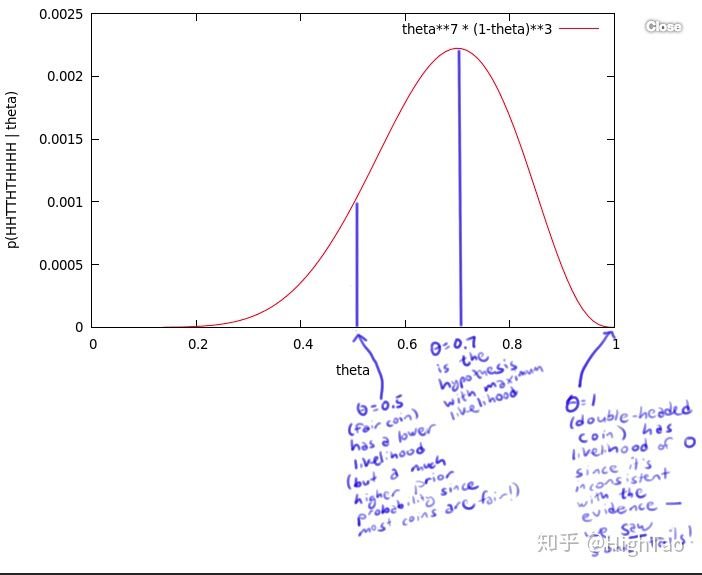
\includegraphics[width=.5\textwidth]{fig/Likelihood_theta_distribution.jpg} %1.png是图片文件的相对路径
  \caption*{$\theta$和概率的关系} %caption是图片的标题
  \label{Likelihood_theta_distribution} %此处的label相当于一个图片的专属标志,目的是方便上下文的引用
\end{figure}

这个曲线就是$\theta$的似然函数,通过了解在某一假设下,已知数据发生的可能性,来评价哪一个假设更接近$\theta$的真实值。如图所示,最有可能的假设是在$\theta = 0.7$的时候取到。但是,你无须得出最终的结论$\theta = 0.7$。事实上,根据贝叶斯法则,0.7是一个不太可能的取值(如果你知道几乎所有的硬币都是均质的,那么这个实验并没有提供足够的证据来说服你,它是均质的)。但是,0.7却是最大似然估计的取值。因为这里仅仅试验了几次,得到的样本太少,所以最终求出的最大似然值偏差较大,如果经过多次试验,扩充样本空间,则最终求得的最大似然估计将接近真实值0.5。

\subsection{贝叶斯定理}
在已知某个参数 B 时,事件 A 会发生的概率记作 $P(A|B)$,有:
$$ P(A|B) = \frac{P(A,B)}{P(B)}$$

利用贝叶斯定理,有:
$$ P(A|B) = \frac{P(B|A)P(A)}{P(B)} $$

反过来,我们可以构造表示似然性的方法:已知有事件 A 发生,运用似然函数:$L(B|A)$,我们来估计参数 B 的可能性。

\section{凸函数}
凸函数:
$$f(tX_1 + (1-t)X_2) <= tf(X_1) + (1-t)f(X_2)$$
其中,$X_1$和$X_2$是 $f(X)$ 定义域 $C$ 上的任意两个点,即$X_1,X_2 \in C$,且 $t \in [0,1]$

严格凸函数:
$$f(tX_1 + (1-t)X_2) < tf(X_1) + (1-t)f(X_2)$$

\section{各种误差函数/损失函数/评价指标}
假设:

预测值:$\hat{y} = {\hat{y_1},\hat{y_2},\cdots,\hat{y_n}}$;

真实值:$y = {y_1, y_2, \cdots, y_n}$;

\subsection{MSE(Mean Square Error)均方误差}
$$MSE = \frac{1}{n}\sum_{i=1}^{n}(\hat{y_i} - y_i)^2$$

均方差损失函数常用在最小二乘法中。它的思想是使得各个训练点到最优拟合线的距离最小(平方和最小)

\subsection{RMSE(Root Mean Square Error)均方根误差}
其实就是 MSE 加了个根号,这样数量级上比较直观,比如 RMSE=10,可以认为回归效果相比真实值平均相差10
$$RMSE = \sqrt{\frac{1}{n}\sum_{i=1}^{n}(\hat{y_i} - y_i)^2}$$

\subsection{MAE(Mean Absolute Error)平均绝对误差}
$$MAE = \frac{1}{n}\sum_{i=1}^{n}|\hat{y_i} - y_i|$$

\subsection{MAPE(Mean Absolute Percentage Error)平均绝对百分比误差}
$$MAPE = \frac{1}{n}\sum_{i=1}^{n}|\frac{\hat{y_i} - y_i}{y_i}|\times 100\%$$

\subsection{MSE均方误差+Sigmoid激活函数\cite{Commonly_Loss_Functions}}
\subsubsection{Sigmoid激活函数}
这个激活函数能将负无穷到正无穷的数映射到0和1之间,表达式和图像为:
$$
\sigma(z) = \frac{1}{1 + e^{-z}}
$$
\begin{figure}[H]
  \centering
  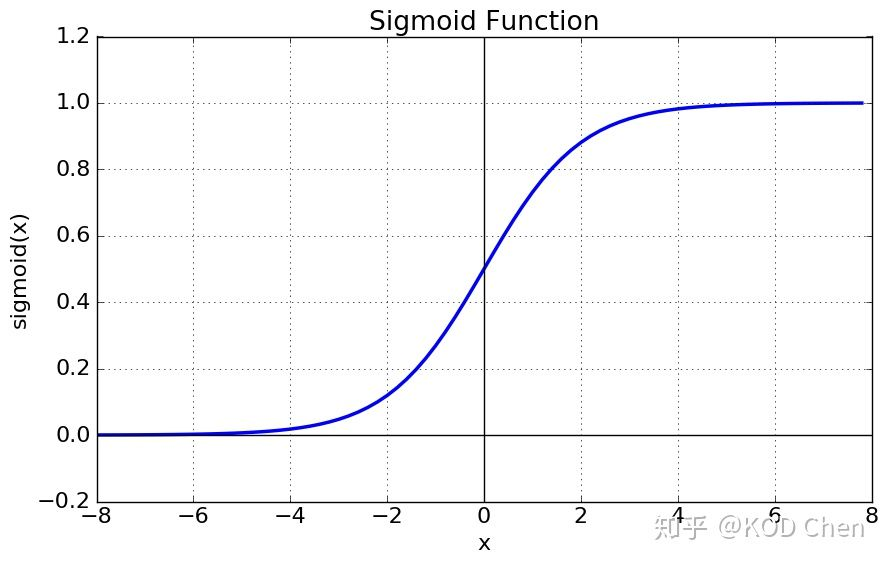
\includegraphics[width=.5\textwidth]{fig/sigmoid_illustration.jpg} 
\end{figure}

Sigmoid的导数推导以及图像:
$$
\sigma'(z) = \frac{0 - 1\cdot(-e^{-z})}{(1+e^{-z})^2} = (1-\sigma(z))\cdot\sigma(z)
$$
\begin{figure}[H]
  \centering
  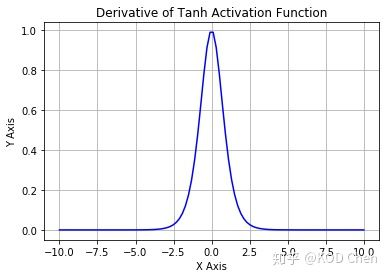
\includegraphics[width=.5\textwidth]{fig/sigmoid_derievative_illustration.jpg} 
\end{figure}

\subsubsection{MSE均方误差+Sigmoid激活函数}
MSE均方误差损失为:$J = \frac{1}{2}(\hat y - y)^2$,Sigmoid激活函数为 $y = \sigma(z) \quad z = wx + b$,可得反向传播过程:
$$
\frac{\partial J}{\partial w} = (\hat y - y)\sigma'(z)x
$$

$$
\frac{\partial J}{\partial b} = (\hat y - y)\sigma'(z)
$$

可以看到最后一层反向传播时,所求的梯度中都含有 $\sigma'(z)$。经过上面的分析,当神经元输出接近1时候,Sigmoid的导数$\sigma'(z)$ 变很小,这样 $\frac{\partial J}{\partial w}$ 、 $\frac{\partial J}{\partial b}$ 很小,这就导致了MSE均方误差+Sigmoid激活函数使得神经网络反向传播的起始位置——输出层神经元学习率缓慢。

\subsection{交叉熵损失(Cross Entropy,CE)\cite{Commonly_Loss_Functions}}
交叉熵多用于分类的损失函数;

\subsubsection{softmax}
交叉熵损失是基于softmax计算来的,softmax将网络最后输出z通过指数转变成概率形式。首先看一下softmax计算公式:
$$
p_i = \frac{e^{z_i}}{\sum_{j=1}^ke^{z_j}}
$$

其中, 分子$e^{z_i}$是要计算的类别 $i$ 的网络输出的指数;分母是所有类别网络输出的指数和,共$k$个类别。这样就得到了类别$i$的输出概率 $p_i$。

实际上,softmax是由逻辑斯的回归模型(用于二分类)推广得到的多项逻辑斯蒂回归模型(用于多分类)。具体可以参考李航大神的《统计学方法》第六章。

\subsubsection{交叉熵损失}
公式定义如下:
$$
J = -\frac{1}{N}\sum_i^N\sum_{i=1}^ky_i\cdot\log{(p_i)}
$$

其中,$y_i$ 是类别 $i$的真实标签$p_i$是上面softmax计算出的类别 $i$ 的概率值;$k$是类别数,$N$是样本总数。

\subsubsection{交叉熵损失+Sigmoid激活函数}
\textbf{推导}:我们仍然以Sigmoid激活函数($y = \sigma(z) \quad z = wx + b$)为例。这次我们引入交叉熵损失,并以二分类为例,那么s损失函数公式为:
$$
J = -\frac{1}{N}[\hat{y}\cdot\ln{y} + (1-\hat{y})\cdot\ln{(1-y)}]
$$

其中:
$$
y = \sigma(z) = \frac{1}{1+e^{-z}} = \frac{1}{1+e^{-(wx+b)}}
$$

那么可以计算一下最后一层的反向传播过程:
$$
\frac{\partial J}{\partial w} = -\frac{1}{N}\sum_1^N[\frac{\hat{y}}{\sigma(z)} - \frac{1-\hat{y}}{1-\sigma(z)}] = \cdots =  -\frac{1}{N}\sum_1^N(\sigma(z)-\hat{y})\cdot x
$$

$$
\frac{\partial J}{\partial b} = -\frac{1}{N}\sum_1^N(\sigma(z)-\hat{y})
$$

\textbf{可以看到sigmoid的导数被约掉,这样最后一层的梯度中就没有$\sigma'(z)$。然而这只是输出层的推导,如果变成隐藏层的梯度sigmoid的导数不会被约掉,仍然存在$\sigma'(z)$。所以交叉熵损失+Sigmoid激活函数可以解决输出层神经元学习率缓慢的问题,但是不能解决隐藏层神经元学习率缓慢的问题。}

\subsection{LearningToRank 中的损失函数\cite{About_RankNet_LambdaRank}}
以文档的相关性排序为例,pairwise算法将排序问题转化为任意两个不同docs $d_i$ 和 $d_j$ 谁与当前query更相关的相对顺序的排序问题,一般分为 $d_i$ 比$d_j$更相关、更不相关和相关程度相等三个类别,分别记为$\{+1, -1, 0\}$,由此便又\textbf{转化为了分类问题}。

若用 $x_i$ 和 $x_j$ 来表示文档 $doc_i$ 和$doc_j$ 的特征$s = f(x;w)$ 代表某种打分函数,$x$和$w$分别代表输入特征和参数。那么文档 $i$ 和 $j$ 的得分为:
$$
s_i = f(x_i;w)
$$
$$
s_j = f(x_j;w)
$$

由于pairwise方法只考虑 $doc_i$ 和$doc_j$ 的相对顺序,\textcolor{red}{RankNet巧妙的借用了sigmoid函数来定义 $doc_i$ 比 $doc_j$ 更相关的概率为:}
$$
P_{ij} = P(doc_i \rhd doc_j) = \frac{1}{1 + e^{-\sigma(s_i - s_j)}}
$$

其中 $\sigma$ 为待学习的参数(其实就是逻辑斯蒂回归)。若$doc_i$ 比 $doc_j$ 更相关,则 $P_{ij} > 0.5$ ,反之$P_{ij} < 0.5$ 。\textcolor{red}{由此便借用了sigmoid函数将 $doc_i$ 比 $doc_j$ 更相关的概率 映射至[0, 1]上的实数,并从概率的角度对“谁更相关”这个问题进行了建模,也让我们得以使用分类问题的思想对两个文档的相对顺序问题进行求解。}

\section{信息熵和信息增益\cite{Book_Machine_Learning_ZhouZhihua}}
\subsection{信息熵}
假定当前样本集合 $D$ 中第 $k$ 类样本所占的比例为 $p_k \quad (k = 1, 2, \cdots, |\mathcal{Y}|)$,则 $D$ 的信息熵定义为:
$$
Ent(D) = -\sum_{k=1}^{|\mathcal{Y}|}p_k\log_2{p_k}
$$

$Ent(D)$ 的值越小,不确定性越小。

\subsection{信息增益}
假定离散属性 $a$ 有 $V$ 个可能的取值 $\{a^1, a^2, \cdots, a^V\}$,若使用 $a$ 来对样本集合 $D$ 进行划分,那么会产生 $V$ 个分直接点,其中第 $v$ 个分直接点包含了 $D$ 中所有在 $a$  上取值为 $a^v$ 的样本,记为 $D^v$,于是我们可以计算出 $D^v$ 的信息熵。再考虑到不同的分支节点所包含的样本数不同,给分支节点赋予权重 $|D^v|/|D|$,即样本数越多的分支节点的影响越大,于是可计算出用属性 $a$ 对样本集$D$进行划分所获得的\textbf{信息增益}:
$$
Gain(D, a) = Ent(D) - \sum_{v=1}^{V}\frac{|D^v|}{|D|}Ent(D^v)
$$

一般而言,我们用信息增益来进行决策树的划分属性选择。即选择属性 $a_*$,使其满足:
$$
a_* = \arg\max_{a \in A}Gain(D,a)
$$

著名的 ID3 决策树学习算法就是以信息增益为准则来选择划分属性。

举个具体的例子:我们有一个包含 17个样本的训练样例$D$,分位两类,即$|\mathcal{Y}| = 2$。在决策树开始学习时,根节点包含$D$中的所有样例,其中正例占 $p_1 = \frac{8}{17}$,反例占 $p_2 = \frac{9}{17}$。于是,可以计算出根节点的信息熵为:
$$
Ent(D) = -\sum_{k=1}^2p_k\log_2{p_k} = -(\frac{8}{17}\log_2\frac{8}{17} + \frac{9}{17}\log_2\frac{9}{17}) = 0.998
$$

然后,我们要计算出当前属性集合(特征)中每个属性(每维特征)的信息增益;以某维特征$a$为例,若用该属性对 $D$ 进行划分,可得到三个子集$D^1, D^2, D^3$,其中子集$D^1$包含有6个样例,其中正例占 $p_1 = \frac{3}{6}$,负例占 $p_2 = \frac{3}{6}$;$D^2$包含有6个样例,其中正例占 $p_1 = \frac{4}{6}$,负例占 $p_2 = \frac{2}{6}$;$D^3$包含有5个样例,其中正例占 $p_1 = \frac{1}{5}$,负例占 $p_2 = \frac{4}{5}$;那么,用该维度特征划分之后所得的三个分支节点的信息熵为:
$$
Ent(D^1) = -(\frac{3}{6}\log_2\frac{3}{6} + \frac{3}{6}\log_2\frac{3}{6}) = 1.000
$$
$$
Ent(D^2) = -(\frac{4}{6}\log_2\frac{4}{6} + \frac{2}{6}\log_2\frac{2}{6}) = 0.918
$$
$$
Ent(D^3) = -(\frac{1}{5}\log_2\frac{1}{5} + \frac{4}{5}\log_2\frac{4}{5}) = 0.722
$$

所以,该属性的信息增益为:
$$
Gain(D,a) = Ent(D) - \sum_{v=1}^3\frac{|D^v|}{|D|}Ent(D^v)
$$
$$
Gain(D,a) = 0.998 - (\frac{6}{17}\times1.000 + \frac{6}{17}\times0.918+\frac{5}{17}\times0.722)
= 0.109
$$

类似的,我们可以计算出每维特征的信息增益,然后选择使得信息增益最大的特征,基于它对根节点进行划分。

\subsection{增益率}
使用信息增益进行特征选择时,对可取值数目较多的属性有所偏好(比如17个样本点的编号 id,取值范围为 1~17)。为了减少这种偏好带来的不利影响,著名的 C4.5决策树算法使用增益率来选择最优划分属性。增益率定义为:
$$
Gain\_ratio(D,a) = \frac{Gain(D,a)}{IV(a)}
$$

其中:
$$
IV(a) = -\sum_{v=1}^V\frac{|D^v|}{|D|}\log_2\frac{|D^v|}{|D|}
$$
称为属性 $a$ 的固有值,属性 $a$ 的可能取值数目越大(即$V$越大),则 $IV(a)$ 的值通常会越大。

注意,增益率准备可能对可取值数目较少的属性有所偏好,因此 C4.5算法并不是直接选择增益率最大的候选划分属性,而是使用了一个启发式方法。

\subsection{基尼系数}
CART 决策树使用基尼系数来选择划分属性。基尼值的定义为:
$$
Gini(D) = \sum_{k=1}^{|\mathcal{Y}|}\sum_{k'\neq k}p_kp_k' = 1 - \sum_{k=1}^{|\mathcal{Y}|}p_k^2
$$

直观来说,$Gini(D)$ 反映从数据集 $D$ 中随机抽取两个样本,其类别标记不一致的概率。因此, $Gini(D)$越小,信息熵越小。

属性 $a$ 的基尼指数定义为:
$$
Gini\_index(D,a) = \sum_{v=1}^{V}\frac{|D^v|}{|D|}Gini(D^v)
$$

\section{正则化方法}
正则化的意义:避免训练得到的模型过拟合(overfitting)训练数据。

\textcolor{red}{过拟合出现时的现象:特征权重 
$W$ 的各个维度的绝对值非常大:一些大整数,一些大负数}。

采用的方式:在损失函数的基础上增加一个关于特征权重 $W$ 的限制,限制它的模不要太大,即:
$$
W = \arg\max_WL(W,Z)
$$
$$
s.t. \psi(W) < \delta
$$

其中,$\psi$ 叫做正则化因子(Regularier),是一个对 $W$ 求模的函数,常用的正则化因子有 L1 和 L2 正则化。

\subsection{L1 正则化}
$$
\psi(W) = ||W||_1 = \sum_{i=1}^N||W_i||
$$

L1正则的本质其实是为模型增加了“\textcolor{red}{模型参数服从零均值拉普拉斯分布}”这一先验知识。证明如下:

TBD

\subsection{L2 正则化}
$$
\psi(W) = ||W||_2^2 = \sum_{i=1}^NW_i^2 = W^TW
$$

L2正则的本质其实是为模型增加了“\textcolor{red}{模型参数服从零均值正态分布}”这一先验知识。证明如下:

TBD

\subsection{为什么 L1 能够产生稀疏解?为什么 L2 能够防止过拟合?\cite{Normalization_Method_L1_L2}\cite{Normalization_In_Machine_Learning}}

\subsubsection{L1}
\begin{align}
     C &= C_0 + \frac{\lambda}{n}\sum_{w}|w| \\
     \frac{\partial C}{\partial w} &= \frac{\partial C_0}{\partial w} + \frac{\lambda}{n}sgn(w) \\
     w^{t+1} &= w^t - \eta\frac{C_0}{\partial w} - \frac{\eta\lambda}{n}sgn(w^t) \\
\end{align}

比原始的更新规则多出了$\frac{\eta\lambda}{n}sgn(w^t)$这一项。当 $w > 0$时,更新后的 $w$ 变小;当 $w < 0$时,更新后的 $w$ 变大——因此它的效果就是让 $w$ 往 0 靠,使网络中的权重尽可能 为 0,所以能够尽可能产生稀疏解;同时也就相当于减小了网络复杂度,防止过拟合。

\subsubsection{L2}
\begin{align}
     C &= C_0 + \frac{\lambda}{2n}\sum_{w}w^2 \\
     \frac{\partial C}{\partial w} &= \frac{\partial C_0}{\partial w} + \frac{\lambda}{n}w \\
     w^{t+1} &= w^t - \eta\frac{C_0}{\partial w} - \frac{\eta\lambda}{n}w^t \\
     &= (1-\frac{\eta\lambda}{n})w^t - \eta\frac{C_0}{\partial w}
\end{align}

在不使用 L2 正则化时,求导结果中 $w$ 前的系数为 1, 使用 L2 正则化后,$w$ 前的系数为 $1-\frac{\eta\lambda}{n}$,因为 $\eta, \lambda, n > 0$,所以 $1-\frac{\eta\lambda}{n} < 1$;它的效果是减小$w$,这也就是权重衰减(weight decay)的由来。当然考虑到后面的导数项,$w$最终的值可能增大也可能减小。

\textbf{为什么 $w$ “变小” 可以防止 overfitting?}

一个所谓“显而易见”的解释就是:更小的权 
$w$ ,从某种意义上说,表示网络的复杂度更低,对数据的拟合刚刚好(这个法则也叫做奥卡姆剃刀),而在实际应用中,也验证了这一点,L2 正则化的效果往往好于未经正则化的效果。

稍微数学一点的解释:过拟合的时候,拟合函数的系数往往非常大,为什么?过拟合,就是拟合函数需要顾忌每一个点,最终形成的拟合函数波动很大。在某些很小的区间里,函数值的变化很剧烈。这就意味着函数在某些小区间里的导数值(绝对值)非常大,由于自变量值可大可小,所以只有系数足够大,才能保证导数值很大。而正则化是通过约束参数的范数使其不要太大,所以可以在一定程度上减少过拟合情况。

\subsection{L1 和 L2 正则化的比较}
L1 在 0 处不可导;L2 可导;但是由于 L1 和 L2 都是凸函数,因此在计算 L1 正则化的梯度方向时,可以采用次梯度代替;

在 Batch 模式下,L1 正则化通常产生更加稀疏的模型,$W$的更多维度为0。这些为 0 的维度代表了不是很相关的维度,从而起到了特征选择的作用;但是在 Online 模式下,每次 $W$ 的更新不是沿着全局梯度进行,即使采用 L1 正则化,也难以产生稀疏解。

\section{避免过拟合的方法}
避免过拟合的方法有很多:early stopping、数据集扩增(Data augmentation)、正则化(Regularization)包括L1、L2(L2 regularization也叫weight decay),dropout。

\section{距离公式}
\subsection{常见的距离公式}
\subsubsection{曼哈顿距离}
点$P_1(x_1, x_2)$和点$P_2(y_1, y_2)$的距离如下:
$$
distance(P_1, P_2) = |x_2 - x_1| + |y_2 - y_1|
$$

\subsubsection{欧氏距离}
点$P_1(x_1, x_2, \cdots, x_n)$和点$P_2(y_1, y_2, \cdots, y_n)$的距离如下:
$$
distance(P_1, P_2) = \sqrt{\sum_1^n(x_i-y_i)^2}
$$

\subsubsection{切比雪夫距离 Chebyshev distance}
二个点之间的距离定义为其各坐标数值差的最大值。点$P_1(x_1, x_2, \cdots, x_n)$和点$P_2(y_1, y_2, \cdots, y_n)$的距离如下:
$$
distance(P_1, P_2) = max(|x_1-y_1|, |x_2-y_2|, \cdots,|x_n-y_n|)
$$

\subsubsection{闵尔科夫斯基距离}
是欧氏距离的推广,是一组距离的的定义。点$P_1(x_1, x_2, \cdots, x_n)$和点$P_2(y_1, y_2, \cdots, y_n)$的距离如下:
$$
distance(P_1, P_2) = \sqrt[p]{\sum_1^n(x_i-y_i)^p}
$$

当$p=1$时,就是曼哈顿距离

当$p=2$时,就是欧式距离

当$p\rightarrow \infty$时,就是切比雪夫距离

\subsubsection{余弦相似度}
余弦相似度是通过测量两个向量夹角的度数来度量他们之间的相似度。结果的测量只与向量的指向方向有关,与向量的长度无关。余弦相似度通常用于正空间,因此给出的值为0到1之间。对于A和B的距离是:
$$
\cos(\theta) = \frac{A\cdot B}{||A||\cdot||B||} = \frac{\sum_1^n(A_i \times B_i)}{\sqrt{\sum_i^n(A_i)^2} \times \sqrt{\sum_i^n(B_i)^2}}
$$

\subsubsection{K-L散度 Kullback-Leibler Divergence}
即相对熵;是衡量两个分布$P$、$Q$之间的距离;越小越相似。
$$
D(P||Q) = \sum_i^nP(i) \log{\frac{P(i)}{Q(i)}}
$$

\subsection{余弦距离探讨\cite{Cosine_Distance}}
\subsubsection{余弦距离}
余弦相似度的取值范围是[-1,1],相同的两个向量之间的相似度为1。如果希望得到类似于距离的表示,将1减余弦相似度即为余弦距离。余弦距离的取值范围为[0,2],相同的两个向量余弦距离为0。
$$
distance(A,B) = 1 - \cos(\theta) = \frac{||A||_2||B||_2 - AB}{||A||_2||B||_2}
$$

\subsubsection{什么要在一些场景使用余弦相似度而不是欧式距离?}
余弦相似度关注的是两个向量之间的角度关系,而\textbf{并不关心它们的绝对大小},其取值范围是[-1,1]。当我们比较两个长度差距很大、但内容相近的文本的相似度时,如果使用词频或词向量作为特征,那么欧式距离会很大;而如果使用余弦相似度,其夹角很小,因而相似度很高。

\subsubsection{余弦距离是否是一个严格定义的距离?}
在一个集合中,如果每一对元素均可唯一确定一个实数,使得三条距离公理(正定性,对称性,三角不等式)成立,则该实数就可称为这对元素之间的距离。

正定性:$d(x,y)>=0$,取等号当且仅当$x=y$

对称性:$d(x,y)=d(y,x)$

三角不等式:$|d(x) - d(y)| <= d(x,y) <= d(x) + d(y)$


\textbf{余弦距离满足正定性和对称性,但是不满足三角不等式}。对于向量A,B:

\textbf{正定性}
\begin{gather*}
    dist(A,B) = 1 - \cos(\theta) = \frac{||A||_2||B||_2 - AB}{||A||_2||B||_2} = \frac{||A||_2||B||_2 - AB}{||A||_2||B||_2} \\
    \because ||A||_2||B||_2 - AB >= 0 \\
    \therefore dist(A,B) >= 0 \\
    \because ||A||_2||B||_2 - AB = 0  \Leftrightarrow A = B \\
    \therefore dist(A,B) = 0 \Leftrightarrow A = B
\end{gather*}

\textbf{对称性}
$$
dist(A,B) = \frac{||A||_2||B||_2 - AB}{||A||_2||B||_2} = \frac{||B||_2||A||_2 - AB}{||B||_2||A||_2} = dist(B,A)
$$

\textbf{三角不等式}

下面给出一个反例:

给定$A=(1,0), B=(1,1), C=(0,1)$,那么:
\begin{gather*}
dist(A,B) = 1 - \frac{\sqrt{2}}{2}   \\
dist(B,C) = 1 - \frac{\sqrt{2}}{2} \\
dist(A,C) = 1 \\
dist(A,B) + dist(B,C) = 2 - \sqrt{2} < 1 = dist(A,C)
\end{gather*}

\textbf{同理,KL距离(又被称为KL散度、相对熵)也不满足对称性和三角不等式}

%\printbibliography
\bibliography{../ref}
\bibliographystyle{IEEEtran}
\end{document}
